\documentclass[
 paper=A4,               % paper size --> A4 is default in Germany
    twoside=true,           % onesite or twoside printing
    openright,              % doublepage cleaning ends up right side
    parskip=full,           % spacing value / method for paragraphs
    chapterprefix=true,     % prefix for chapter marks
    11pt,                   % font size
    headings=normal,        % size of headings
    bibliography=totoc,     % include bib in toc
    listof=totoc,           % include listof entries in toc
    titlepage=on,           % own page for each title page
    captions=tableabove,    % display table captions above the float env
    draft=false,            % value for draft version
]{scrreprt}

\usepackage{newstyle}
\usepackage{tabularx}
\usepackage[utf8]{inputenc}
\usepackage{amsmath,amsfonts,amssymb,amsthm,url}
\def\UrlBreaks{\do\/\do-}
\usepackage[portuguese,english]{babel}
\usepackage{times}
\usepackage{setspace}
\usepackage[sort&compress,numbers]{natbib}
\usepackage[vlined,ruled,commentsnumbered,linesnumbered]{algorithm2e} 
\usepackage{algorithmic}  
\usepackage{graphicx,multirow}
\usepackage{array}
\usepackage{multicol}
\usepackage{mathptmx} % use Times in math mode
%\usepackage{moreverb}
\usepackage{lscape,rotating}
\usepackage{hyperref}
\usepackage{fancyhdr}
\usepackage{lastpage}
\usepackage{nameref}
\usepackage{listings}
\usepackage{subfig}
\usepackage{tikz}
\usepackage{xcolor}
\usepackage{makeidx}
\usepackage{epsfig}
\usepackage{xspace}
%\usepackage{subfigure}
%\usepackage[show]{chato-notes}
%\usepackage{listings}
\usepackage{color}
\usepackage{marginnote}
\usepackage{flushend}
\usepackage{breakurl}
\usepackage{lipsum}  

\makeindex


\theoremstyle{definition}
\newtheorem{defn}{Definition}[]

\newcommand*\circled[1]{\tikz[baseline=(char.base)]{
            \node[shape=circle,fill,inner sep=1pt] (char) {\textcolor{white}{#1}};}}

\fancyhf{} %
\lhead{\nouppercase {\leftmark}} %
\rhead{\nouppercase {\bf \thepage}}
\renewcommand{\headrulewidth}{0.1pt}

% Comando para inserir pagina em branco (inserida na numeracao, mas sem
% numero impresso) para quando e' preciso obrigar um capitulo a comecar
% do lado direito (pagina impar)
\newcommand{\LIMPA}{
\newpage
\mbox{}
\thispagestyle{empty}
}

% Igual, mas insere pagina com numero impresso (normalmente nao se usa)
\newcommand{\LIMPAC}{
\newpage
\mbox{}
\thispagestyle{plain}
}

%
% ALTERAR AQUI AS INFORMACOES RELATIVAS AO PROJECTO
%
\newcommand{\TITULO}{TITULO DO TRABALHO}
\newcommand{\Autor}{NOME DO ALUNO}
\newcommand{\AutorNumAluno}{NUMERO DO ALUNO}

%Orientador e CoOrientador *sem* titulos (e.g. Prof. Doutor)
\newcommand{\Orientador}{NOME ORIENTADOR}
\newcommand{\CoOrientador}{NOME CO-ORIENTADOR} %se nao se aplicar, nao importa o que aqui esteja

%Se aplicavel, o supervisor pode ter um titulo (Dr., Eng.) colocado aqui
\newcommand{\SupervisorInstituicao}{Nome Completo do Supervisor}  %se nao se aplicar, nao importa o que aqui esteja

\newcommand{\AnoLectivo}{2019/2020}
\newcommand{\Ano}{\Large{2020}}

% Comentar/descomentar conforme conveniente
\newcommand{\CADEIRA}{Trabalho Final de Curso}

% Comentar/descomentar conforme conveniente
%\newcommand{\IdiomaTese}{\selectlanguage{portuguese}}
\newcommand{\IdiomaTese}{\selectlanguage{english}}


\newcommand{\Cabecalho}{
\vspace{-0.5cm}\normalfont\normalfont
\vfill
\textsc{\normalsize\uppercase{Instituo Superior Manuel Teixeira Gomes}}\\
\vspace{1.5cm}

\includegraphics[scale=.9]{pic/logotipo_ISMAT.pdf}\\
}


\title{\TITULO}
\author{\Autor}
%\date{\today}

\usepackage{glossaries}
\makeglossaries

\begin{document}
\selectlanguage{english}
\pagestyle{empty}

% Primeira capa
% 
%
\begin{center}

\Cabecalho

\vspace{2.0cm}
\vfill
\IdiomaTese
\Large{\textbf{\TITULO}}\\
\vspace{1cm}
\vfill

\large{\textbf{\CADEIRA}}\\
\vspace{1.0cm}
\vfill
\Large{\textbf{\Autor}}\\
\vspace{1,8 cm}
\vfill
\large{Trabalho orientado por:}\\
\large{Prof. \Orientador} \\
% DESCOMENTAR a linha relevante (se alguma), removendo o % no inicio
e pelo Prof. \CoOrientador \\
\vspace{1 cm}
\vfill

\vspace{0.5cm}
\vfill
\vspace{-1cm}
\Ano
\end{center}


% Fim da capa
% ----------------------------------------------------------------------

\pagenumbering{roman}			% roman page numbing (invisible for empty page style)
\setcounter{page}{1}			% set page counter
\pagestyle{empty}

%\cleardoublepage

%\pagestyle{plain}

\vspace*{2cm}
\selectlanguage{portuguese}
\chapter*{Agradecimentos}

\lipsum[1-3]


\selectlanguage{english}


\LIMPA


\pagestyle{plain}				% display just page numbers
% ----------------------------------------------------------------------
% P�gina do resumo em Ingl�s:
% 300 palavras
\selectlanguage{english}
%\vspace*{2cm}
%\begin{center}
%\Large \bf Abstract
%\end{center}
%\vspace*{1cm} \setlength{\baselineskip}{0.6cm}
\chapter*{Abstract}
\label{chapter:abstract_en}
\vspace*{-10mm}
\lipsum[1-3]

\vfill

\begin{flushleft}
\textbf{Keywords:}
Keyword1, Keyword1, Keyword3, Keyword4, Keyword5.
\end{flushleft}

%\LIMPA

% Fim da p�gina do resumo em Ingl�s.
% ----------------------------------------------------------------------

%\cleardoublepage



%Lista de capitulos
\setcounter{secnumdepth}{3}
\setcounter{tocdepth}{2}		% define depth of toc
\tableofcontents				% display table of contents
%\addcontentsline {toc} {chapter} {Content}
\newpage
\thispagestyle{empty}
\mbox{}
\newpage


%Lista de figuras
\listoffigures
%\addcontentsline {toc} {chapter} {List of Figures}
\newpage
%\thispagestyle{empty}
%\mbox{}
%\newpage

%Lista de tabelas
\listoftables
%\addcontentsline {toc} {chapter} {List of Tables}
\newpage
%\thispagestyle{empty} \mbox{}
%\newpage

%
% Para actualizar o glossario, e' preciso correr o script ./fazindice
% e voltar a gerar o PDF
%
%\LIMPA
%\renewcommand{\glossaryname}{Acronyms}
%% abbreviations:
\newacronym{nasa}{NASA}{National Aeronautics and Space Administration}

%\printglossaries
%\addcontentsline {toc} {chapter} {Acronyms}
% Bibliografia

% --------------------------
% Body matter
% --------------------------

% ----------------------------------------------------------------------
% Inicio conteudo
\pagestyle{fancy}
\cleardoublepage

%\setcounter{page}{1}
%\pagenumbering{arabic}

\pagenumbering{arabic}			% arabic page numbering
\setcounter{page}{1}			% set page counter
\pagestyle{maincontentstyle} 		% fancy header and footer



\chapter{Introduction}
\label{chap:introduction}
\lipsum[1-3]


This is a citation example~\cite{Garcia:2018}

\gls{nasa} is an acronym example. \gls{nasa} is cool.

\begin{figure}[!t]
\begin{center}
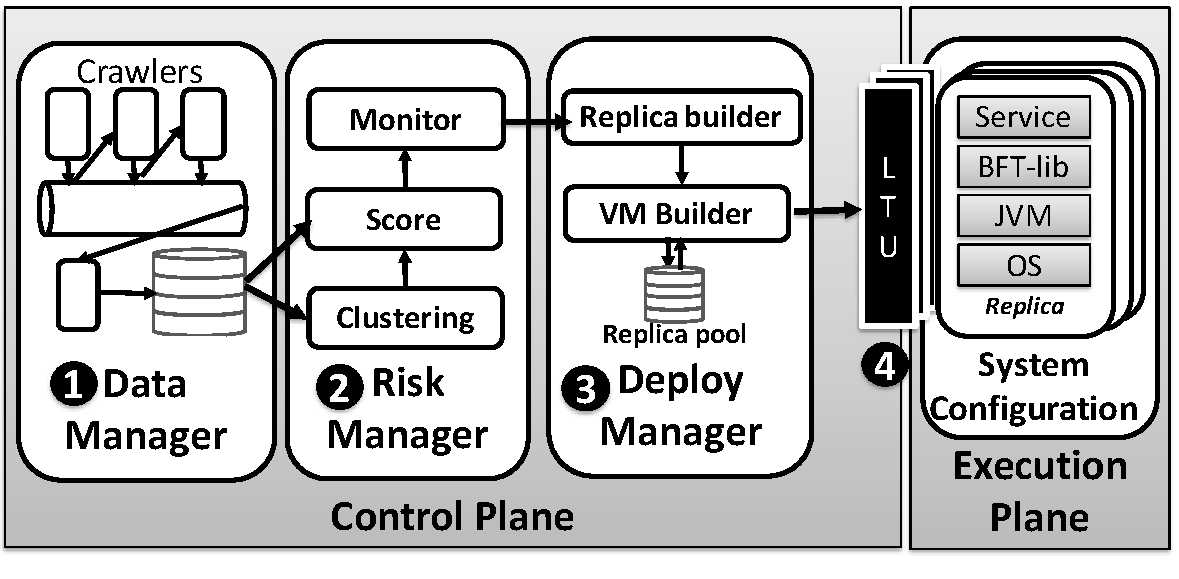
\includegraphics[width=\columnwidth]{images/figure_example.pdf}
%\vspace{-5mm}
\caption{This is figure example.}
\label{fig:overview}
\end{center}
\end{figure}



This is an equation Example
\begin{equation} 
\begin{split}
\textit{oldness}(v)=\\\textit{max}\left((1-0.25\times\frac{(\textit{now}-v.\textit{published\_date})}{\textit{oldness\_threshold}}), 0.75\right)
\label{eq:oldness}
\end{split}
\end{equation}

\begin{algorithm}[H]
\SetAlgoLined
\KwResult{Write here the result }
 initialization\;
 \While{While condition}{
  instructions\;
  \eIf{condition}{
   instructions1\;
   instructions2\;
   }{
   instructions3\;
  }
 }
 \caption{Algorithm example}
\end{algorithm}



\begin{table}[!t]
\begin{center}
{\footnotesize
\begin{tabular}{| l | l | c | c |}\hline
\textbf{ID} & \textbf{Name}  & \textbf{\#Cores} & \textbf{Memory}  \\\hline\hline
UB14 & Ubuntu 14.04 & 4 & 15GB  \\ \hline
UB16 & Ubuntu 16.04 & 4 & 15GB \\ \hline
UB17 & Ubuntu 17.04 & 4 & 15GB\\ \hline
OS42 & OpenSuse 42.1 & 4 & 15GB \\ \hline
FE24 & Fedora 24 & 4 & 15GB  \\ \hline
FE25 & Fedora 25 & 4 & 15GB  \\ \hline
FE26 & Fedora 26 & 4 & 15GB \\ \hline
\end{tabular}
}
\caption{TABLE EXAMPLE}
\label{tab:oses}
\end{center}
\end{table}





% Fim do conteudo
% ----------------------------------------------------------------------

% Glossario

\LIMPA
\bibliographystyle{abbrv}
\bibliography{chapters/references/references}
%\addcontentsline {toc} {chapter} {Bibliography}

\end{document}

